\documentclass[class=ctexart,crop=false]{standalone}

\usepackage{amsmath,amssymb,enumitem,empheq,tkz-euclide,
diagbox,wrapfig,pgfplots,geometry}
%\geometry{a4paper,scale=0.9}
\pgfplotsset{compat=newest}
%\usepgfplotslibrary{external}
%\tikzexternalize
\renewcommand\parallel{\mathrel{/\mskip-2.5mu/}}

\newcommand\px{\mathrel{/\mkern-5mu/}}  %平行
\newcommand\pxeq{\mathrel{\vcenter{     %平行且等于
\ialign{\hfil##\hfil\crcr
$\scriptstyle\px\!$\crcr
\noalign{\nointerlineskip\vskip1pt}$=$\crcr}}}}

%\setCJKmainfont{SimSun}       %设置西文字体为times new roman
%\setCJKsansfont{SimSun}             %设置中文字体为宋体
%\setCJKmonofont{STKaiti}
%\setsansfont{TeX Gyre Termes}            %设置typewriter family中文字体为楷体
%\setmonofont{TeX Gyre Termes}

\usetikzlibrary{calc,intersections,through,backgrounds,patterns}
\newcounter{para}
\newcommand\mypara{\par\refstepcounter{para}\thepara.\space}%设置typewriter family西文字体为times new roman
\newcommand*\circled[1]{\tikz[baseline=(char.base)]{
            \node[shape=circle,draw,inner sep=1pt] (char) {#1};}}

\newcommand{\rnum}[1]{\romannumeral #1}
\newcommand{\RNum}[1]{\uppercase\expandafter{\romannumeral #1\relax}}
\begin{document}
解:截取任一圆锥高所在平面,由旋转对称性,球最大时该截面截球所得圆恰为截圆锥所得三角形内接圆\\
如图,易知 $h=\sqrt{3^2-1^2}=2\sqrt{2},$\\
$r^2+AE^2=(2\sqrt{2}-r)^2$\\
$r^2+2^2=r^2+8-4\sqrt{2}r$\\
$r=\frac{\sqrt{2}}{2}$\\
$V=\frac{4\pi r^3}{3}=\frac{4}{3}\times  \frac{\sqrt{2}}{2}\times\frac{1}{2} \pi=\frac{\sqrt{2}\pi}{3}$\\
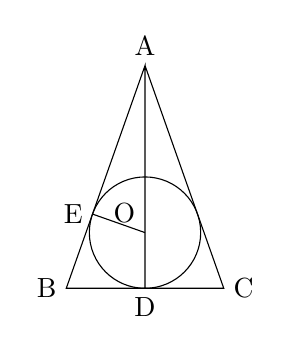
\begin{tikzpicture}
    \coordinate [label={90:{A}}] (A) at ($sqrt(2)*(0,2)$) {};
    \coordinate [label={180:{B}}] (B) at (-1,0) {};
    \coordinate [label={0:{C}}] (C) at (1,0) {};
    \coordinate [label={270:{D}}] (D) at (0,0) {};
    \coordinate [label={120:{O}}] (O) at ($sqrt(2)*(0,0.5)$)  {};
    \draw (D)--(A)--(B)--(C)--(A);
    \node [draw] (oo) at  (O) [circle through={(D)}] {};
    \coordinate[label={180:{E}}] (E) at (intersection 1 of oo and B--A);
    \draw (E)--(O);
\end{tikzpicture}
\end{document}